\documentclass[12pt]{article}

% Packages for enhanced functionality
\usepackage{graphicx}      % For including images
\usepackage{caption}       % For customizing captions
\usepackage{amsmath}       % For mathematical symbols and environments
\usepackage{geometry}      % To adjust page margins
\usepackage{float}         % For improved figure placement
\usepackage{hyperref}      % For hyperlinks within the document

% Page layout settings
\geometry{
	a4paper,
	left=25mm,
	right=25mm,
	top=25mm,
	bottom=25mm
}

% Document metadata
\title{Project 1 - Part 1}
\author{Adil Hydari}
\date{\today}

\begin{document}
	
	% Title Page
	\maketitle
	
	
	% Plot Section
	\section{Memory Bandwidth vs. Region Size}
	
	% Figure Environment with the Plot
	\begin{figure}[H]
		\centering
		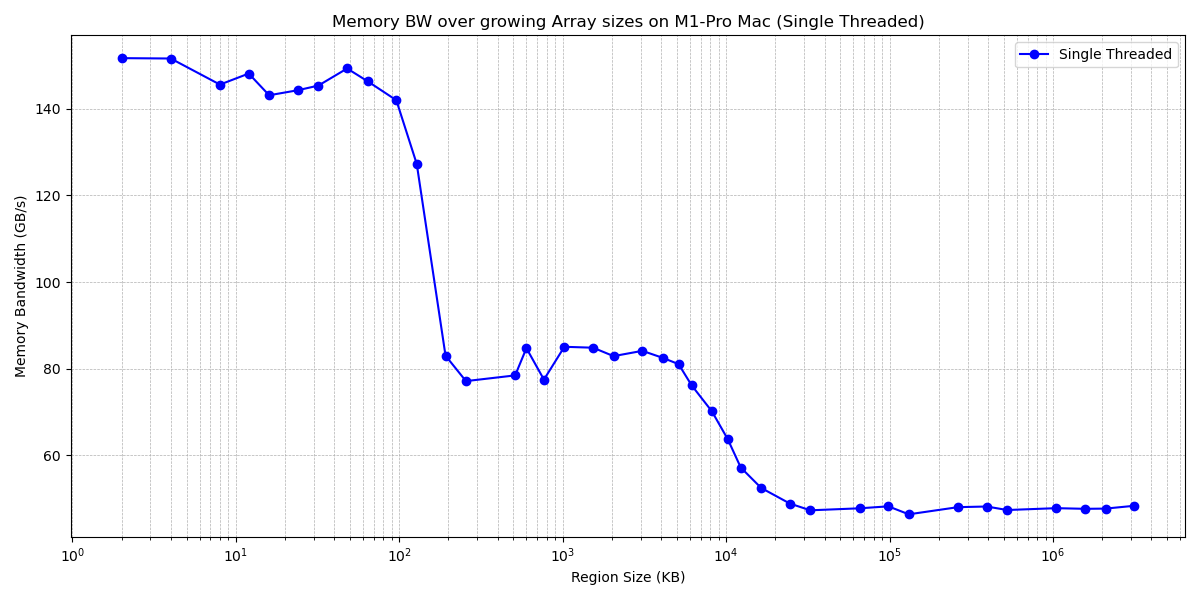
\includegraphics[width=\linewidth]{memory_bandwidth_gbps.png}
		\caption{Memory Bandwidth as a Function of Region Size (Single-Threaded)}
		\label{fig:memory_bandwidth}
	\end{figure}
	
	% Explanation Subsection
	\subsection{Analysis of the Plot}
	Figure \ref{fig:memory_bandwidth} illustrates the relationship between region size (measured in kilobytes, KB) and memory bandwidth (measured in gigabytes per second, GB/s) on a single-thread. The region sizes range from 2 KB to ~3 GB
	
	\subsubsection{Observations}
	\begin{itemize}
		\item \textbf{Initial:} For region sizes up to approximately 32 KB, memory bandwidth remains relatively high and stable, hovering around 145 GB/s. This stability suggests that data within these array sizes, is directly being handled by the cache, allowing for the highest bandwidth.
		
		\item \textbf{Bandwidth Decline:} As the region size increases beyond the cache capacities (i.e. beyond 128 KB), there is a decline in memory bandwidth, dropping to around 47 GB/s for the largest region sizes. This decline indicates a transition from cache-based access to main memory access (DRAM), which offers lower bandwidth.
		
		\item \textbf{Larger Sizes:} Beyond a ~131,072 KB and above, the memory bandwidth plateaus, suggesting that further increases in region size do not significantly impact bandwidth, as the system is already relying primarily on main memory.
	\end{itemize}
	
	% Conclusion Section
	\section{Conclusion}
	The analysis shows a clear relationship between region size and memory bandwidth in a single-threaded environment. Smaller region sizes benefit from high memory bandwidth due to efficient cache utilization, while larger region sizes incur reduced bandwidth as they rely on slower main memory access.
	
	% References (Optional)
	\begin{thebibliography}{9}
		\bibitem{memory_hierarchy} 
		John L. Hennessy and David A. Patterson, \textit{Computer Architecture: A Quantitative Approach}, 5th Edition, Morgan Kaufmann, 2011.
		
		\bibitem{Memory Bandwidth code reference} 
		My code is based on: \href{https://github.com/ChipsandCheese/Microbenchmarks}{Microbenchmarks}
		
	\end{thebibliography}
	
\end{document}
